\documentclass{article}
\usepackage{tikz}
\usetikzlibrary{arrows,decorations.pathmorphing,backgrounds,positioning,fit,petri}
\begin{document}
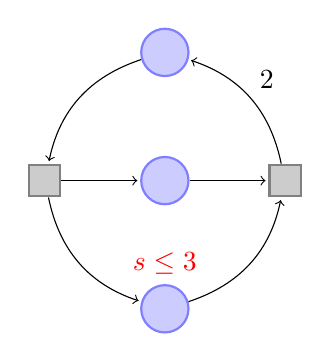
\begin{tikzpicture}[
    place/.style={circle,draw=blue!50,fill=blue!20,thick,
        inner sep=0mm,minimum size=6mm},
    transition/.style={rectangle,draw=black!50,
        fill=black!20,inner sep=0mm,minimum size=4mm,thick},
    every label/.style=red
]
 \node[place] (waiting) {};
 \node[place] (critical) [below=of waiting] {};
 \node[place] (semaphore) [below=of critical,label=above:$s\le3$] {};
 
 \node[transition] (leave critical) [right=of critical] {}
    edge[pre] (critical)
    edge[post,bend right] node[auto,swap] {$2$} (waiting)
    edge[pre,bend left] (semaphore);
 \node[transition] (enter critical) [left=of critical] {}
    edge[post] (critical)
    edge[pre,bend left] (waiting)
    edge[post,bend right] (semaphore);
\end{tikzpicture}
\end{document}

